% IEEE TIM submission draft.
% Requires IEEEtran.cls (journal mode) and the standard graphicx/booktabs/amsmath set.
\documentclass[journal]{IEEEtran}
\usepackage{amsmath,amssymb,booktabs,graphicx,array}
\usepackage{cite}
\usepackage[colorlinks=false,hidelinks]{hyperref}
\graphicspath{{../figures/tim/}}

\newcommand{\dx}{\delta^{\star}}
\newcommand{\EAC}{\textsc{eac}}

\begin{document}

\title{What a Remaining-Useful-Life Interval Can Prove: Coverage, Width, and the Calibration Object}

% ---------------------------------------------------------------- author block
% TODO before submission: replace the two lines below with the real author list,
% affiliations and funding note.  Nothing else in the file needs to change.
\author{Author names withheld in this draft% <- fill in before submission
\thanks{Manuscript prepared 2 November 2026. Affiliations and funding to be added.}}

\maketitle

\begin{abstract}
Prediction intervals for remaining useful life (RUL) are reported as a coverage rate close to
nominal and a width as small as possible. This paper asks how much of that pair is information
and how much is convention, using 653 test engines from the four C-MAPSS fleets and 2\,587
cycle-level queries from N-CMAPSS. Three conventions are isolated and priced. First, scoring
coverage on the integer grid inflates PICP by $+0.011$ to $+0.044$ at the 90\,\% level and by
$+0.074$ to $+0.120$ at 50\,\%, independent of the model; randomised PIT removes the shift.
Second, reporting the \emph{central} interval of a predictive distribution rather than the
\emph{shortest} interval of the same mass costs 10.4\,\% of the width (30.9 $\rightarrow$ 27.7
cycles) at identical coverage. Third, calibrating a cross-validation fold model while deploying
an ensemble --- the standard CV+ construction --- costs a further 11\,\% (35.3--36.3
$\rightarrow$ 31.4--32.4 cycles). A matched-object construction that calibrates the deployed
ensemble reaches 32.4 cycles against the 30.9 of a 66-parameter parametric layer, with
$|\Delta| = 0.014$ across fleets where the layer ranges 0.842--0.932. An uncalibrated
fifteen-member deep ensemble covers 0.485--0.553 at nominal 0.90, and conformalised quantile
regression 0.883--0.919 at 14--22\,\% more width. With 11--82 engines per RUL bin, the smallest
detectable coverage deviation is 0.14--0.44; 149 engines per bin are needed to detect 0.10.
N-CMAPSS returns 0.896 and 0.493, and a simulation with known truth confirms nominal coverage
across 50--2\,000 calibration engines.
\end{abstract}

\begin{IEEEkeywords}
Remaining useful life, uncertainty quantification, conformal prediction, calibration,
coverage, measurement uncertainty, prognostics and health management.
\end{IEEEkeywords}

\section{Introduction}

A remaining-useful-life (RUL) predictor that returns a single number cannot be used to
schedule maintenance: the planner needs to know how wrong the number may be. The literature
has therefore converged on interval-valued prognostics \cite{angelopoulos2023,kuleshov2018}, reported through two statistics ---
the fraction of engines whose true RUL falls inside the interval (PICP), and the mean interval
width. The implicit claim is that the first is at least the nominal level and the second is as
small as the method can make it.

Recent work in this journal has advanced that programme considerably. CRULP combines
conformalised quantile regression with cross-conformal prediction to turn a point predictor
into an interval with a distribution-free guarantee \cite{crulp}, and related studies extend
conformal RUL to covariate shift \cite{piao2025}, to missing and faulty sensor data
\cite{wang2025}, and to IoT predictive maintenance \cite{moccardi2025}. The methodological
question these papers raise is no longer \emph{whether} a guarantee can be attached to an RUL
interval. It can. The question is what a specific experiment on a specific benchmark can
\emph{show} about the interval it reports.

A parallel literature improves the predictor rather than the interval: evidential and
domain-adaptive formulations that carry their own uncertainty \cite{hou2025}, bearing
prognostics that pair a degradation indicator with a Bayesian network \cite{yang2025},
model-based degradation models that derive the first-hitting-time density analytically
\cite{wang2025svsdm}, architecture work on the turbofan benchmarks \cite{kim2025}, and
conformal active learning that uses the interval width to choose what to label
\cite{wu2025}; \cite{zhou2025} surveys the health-indicator branch. Two features of that body
of work matter here. Most of it reports either a predictive density or an interval, and the
convention that converts one into the other is rarely stated, although it moves the reported
score by up to 0.12 (Section~\ref{sec:measure}). And the uncertainty is usually validated by a
coverage number computed on the same benchmark, which at these sample sizes cannot resolve
differences below 0.14 (Section~\ref{sec:measure}).

This paper takes that question literally and answers it with measurements rather than
arguments. We hold the backbone fixed (a 41\,858-parameter model, five folds, three seeds),
hold the test engines fixed (653 engines for C-MAPSS, 2\,587 queries over 39 units for
N-CMAPSS), and vary only the construction of the interval. Five results follow, and each is a
number rather than a preference.

\begin{enumerate}
\item \textbf{Coverage is measured with a biased instrument.} RUL is a lattice-valued target
capped at 125 cycles. Reporting an interval by its integer endpoints counts a hit whenever the
endpoints straddle the truth, which adds the mass that lies between the endpoint and the
quantile it was meant to represent. The bias is $+0.011$ to $+0.044$ at nominal 0.90 and
$+0.074$ to $+0.120$ at nominal 0.50 on the four fleets, always positive, and has nothing to
do with the predictor. Randomised PIT removes it.
\item \textbf{The benchmarks cannot resolve the differences they are used to rank.} With
11--82 engines in an RUL bin, a binomial test at family-wise 5\,\% detects only deviations of
0.14--0.44 at 80\,\% power. Detecting a 10-point deviation needs 149 engines per bin, and a
5-point deviation needs 516. At the fleet level the 95\,\% band on a coverage of 0.90 is
$\pm 0.060$ ($n=93$) to $\pm 0.038$ ($n=235$), which is of the same order as the differences
between methods that published tables rank.
\item \textbf{Two construction choices each cost about a tenth of the width.} The central
interval of a predictive distribution is not the shortest interval of the same mass; on the
frozen layer the shortest-interval rule saves 10.4\,\% of the width at identical coverage.
Calibrating the fold model rather than the deployed ensemble costs 11\,\% in the CV+
construction.
\item \textbf{A matched construction closes the gap to a parametric layer without its
assumptions.} Calibrating on residuals of the object that is actually deployed, with signed
scores and a free tail allocation, gives 32.4 cycles against the layer's 30.9 on the same
engines, with coverage $0.897$--$0.925$ against the layer's $0.842$--$0.932$.
\item \textbf{Uncalibrated deep ensembles are the largest error in the comparison.} A
fifteen-member ensemble reported as $\mu\pm z_{0.95}\sigma$ covers 0.485--0.553 at nominal
0.90. Conformalising a quantile regression on the same engines repairs most of that
(0.883--0.919) but is 14--22\,\% wider than the matched construction.
\end{enumerate}

The remainder of the paper is organised as follows. Section~\ref{sec:measure} formalises what
a coverage number can resolve. Section~\ref{sec:construct} defines the constructions and their
guarantees. Section~\ref{sec:protocol} fixes the experimental protocol.
Section~\ref{sec:results} reports results on C-MAPSS, N-CMAPSS and a controlled simulation.
Section~\ref{sec:discussion} discusses what should be reported, and Section~\ref{sec:concl}
concludes.

\section{What a Coverage Number Can Resolve}\label{sec:measure}

\subsection{Two ways to score the same distribution}

Let $F_i$ be a predictive distribution over the integer grid $\{0,\dots,K\}$, $K=125$, and let
$Y_i$ be the realised RUL. An interval $[L_i,U_i]$ covers when $L_i \le Y_i \le U_i$. Two
conventions are in use.

\emph{Integer endpoints.} $L_i$ and $U_i$ are integers, and coverage is the empirical
frequency of $L_i \le Y_i \le U_i$.

\emph{Randomised PIT.} Draw $V_i \sim \mathrm{U}(F_i(Y_i-1), F_i(Y_i))$ and count
$V_i \in [(1-\tau)/2, (1+\tau)/2]$. This is the probability integral transform evaluated
inside the atom that contains the observation, and it is unbiased for the nominal level of a
\emph{continuous} interval on the same distribution.

The two agree only when the pmf is smooth relative to the grid. For a RUL distribution that is
censored at $K$ --- where 17\,\% of the C-MAPSS engines sit exactly at 125 --- the endpoint rule
adds the atom and part of the neighbouring bin to every interval whose endpoint lands there.
Writing $b_i$ for that surplus mass,
\begin{equation}
\widehat{\mathrm{PICP}}_{\text{int}} - \widehat{\mathrm{PICP}}_{\text{PIT}}
= \frac1n\sum_i b_i \;\ge\; 0,
\end{equation}
so the bias is one-sided and its size is set by how concentrated the pmf is near the endpoints.
Table~\ref{tab:convention} reports it: 0.011--0.044 at 0.90 and 0.074--0.120 at 0.50.
The layer discussed in Section~\ref{sec:results} would be reported as well calibrated
(0.886--0.948) under the integer rule and as under-covering (0.842--0.932) under randomised
PIT. Both numbers describe the same object.

\subsection{What \texorpdfstring{$n$}{n} engines can detect}

A coverage claim is a hypothesis test. For a bin holding $n$ engines whose true coverage is
$p_0=\tau$, the exact two-sided binomial test at level $\alpha$ rejects when the count falls
outside its acceptance region. The smallest $p_1<\tau$ detected with power $1-\beta$ is
\begin{equation}
\begin{aligned}
\dx(n) &= \tau - \max\{p : \Pr[\mathrm{Bin}(n,p)\le c_\alpha] \ge 1-\beta\},\\
c_\alpha &= \lfloor \mathrm{Bin}^{-1}(\alpha/2; n,\tau)\rfloor .
\end{aligned}
\end{equation}
The quantity depends only on how many engines fall in the bin and on the nominal level; it is
independent of the predictor, the backbone and the interval construction. It is therefore a
property of the \emph{benchmark}, not of the method, and it bounds what any method comparison
on that benchmark can conclude. Table~\ref{tab:detect} evaluates it at the five RUL bins used
in this paper, with a Bonferroni correction over the five bins.

\subsection{Paired comparisons}

Two intervals scored on the same engines are paired, so the relevant noise is the discordance
count rather than the marginal standard error. We report McNemar's exact test for this. It
matters because a difference of 0.03 in marginal coverage can be produced by 3 engines out of
100, while the paired version of the same difference may be significant or not depending on
whether the methods err on the same engines.

\section{Constructing the Interval}\label{sec:construct}

\subsection{Scores}

Let $\hat y_i$ be the point prediction of the deployed model and $R_i = y_i - \hat y_i$ a
signed residual. Two score families are standard.

\emph{Equal length.} Use $s_i = |R_i|$, take $q$ the $\lceil(1-\alpha)(n+1)\rceil$-th smallest
score, and report $[\hat y - q, \hat y + q]$. The interval is symmetric about the prediction by
construction.

Conformalised quantile regression \cite{romano2019} learns the two quantiles with a pinball
loss instead of taking them from a residual sample; it is the construction used by the
closest prior work \cite{crulp}, and the two are equivalent when the quantile model is
well specified. We use the residual form because it isolates the effect of the score.

\emph{Free tails.} Use the signed residuals directly and report
$[\hat y + q_{\gamma}, \hat y + q_{1-\alpha+\gamma}]$ with $\gamma \in [0,\alpha]$. Setting
$\gamma=\alpha/2$ gives equal-tailed probability; setting $\gamma$ to minimise
$q_{1-\alpha+\gamma}-q_\gamma$ gives the shortest interval of mass $1-\alpha$ in the family.

The two families coincide when the residual law is symmetric, and differ otherwise. Which one
is narrower is an empirical question about the residual law, not a theorem: a sharply peaked
law can favour equal length (the $90$th percentile of $|R|$ is below the $95$th percentile of
$R$), while a diffuse or skewed law favours free tails. Section~\ref{sec:results} reports both
signs.

\subsection{Shortest versus central}

For a predictive distribution rather than a score sample --- the case of the parametric layer
here, and of the analytically derived first-hitting-time densities in
\cite{wang2025svsdm} --- the analogue of the choice is between the central interval, defined
by equal tail mass, and the shortest interval of mass $\tau$,
\begin{equation}
[L_i,U_i] = \arg\min_{a \le b}\;(b-a)\ \ \text{s.t.}\ \ F_i(b)-F_i(a^-) \ge \tau .
\end{equation}
The two coincide only for symmetric unimodal pmfs. For a censored RUL pmf they do not, and the
gap is a pure convention cost: the coverage of the pair is identical because both contain mass
$\tau$ of the same distribution.

\subsection{Which object is calibrated?}

Split conformal \cite{vovk2005} with a calibration set of size $m$ guarantees
$\Pr[Y \in [L,U]] \ge 1-\alpha$ for exchangeable data, with the finite-sample correction used
above. CV+ \cite{barber2021} extends the guarantee to the case where the predictor must be
trained on the same data that calibrates it: for each calibration point $i$ held out by fold
$k(i)$, the endpoint set is $\{\hat y_{-k(i)}(x) + R_i\}$, and the interval is a quantile of
that set. Barber et al.\ prove coverage $\ge 1-2\alpha$ for this construction.

The construction calibrates the object $\hat y_{-k}$, a model trained on a $(1-1/K)$ fraction
of the data. If what is deployed is the average of the $K$ fold models --- the natural choice,
and the one used by every ensemble in this paper --- then the calibrated object and the
deployed object differ by exactly the fold spread. The interval inherits that spread as a
fixed width penalty in cycles, which is invisible at $\tau=0.90$ and dominant at $\tau=0.50$.

\emph{Matched object.} With repeated cross-fitting the mismatch can be removed at no extra
cost. If the same partition is used for $S$ seeds, engine $i$ in fold $k$ is excluded from
$S$ models, one per seed, and their average is an ensemble that has never seen $i$. Calibrating
on the residuals of that ensemble and centring on the full $K\times S$ ensemble gives a score
whose law matches the deployed object up to the ensemble size ($S$ versus $KS$ members).

We call the resulting construction \EAC{} (ensemble-aware conformal): matched-object residuals,
signed scores, optional variance normalisation, and a tail allocation $\gamma$ chosen to
minimise the empirical width. Each component is ablated in Section~\ref{sec:results}.

\subsection{Guarantees and what they do not cover}

For exchangeable calibration and deployment data, split conformal gives
$\Pr[Y\in[L,U]] \ge 1-\alpha$ for any fixed $\gamma$, so the tail allocation cannot invalidate
the guarantee; choosing $\gamma$ from the same sample adds a second-order selection effect,
measured in Section~\ref{sec:results} at 0.003--0.006 in coverage. The guarantee is marginal:
it says nothing about coverage conditional on the predicted RUL, and
Section~\ref{sec:measure} shows that on these benchmarks nothing could.

\section{Protocol}\label{sec:protocol}

\subsection{Data}

\emph{C-MAPSS} \cite{saxena2008}: four fleets (FD001--FD004), 100 training engines each, and
93/235/97/228 test engines, 653 in total. Each test engine contributes one query, taken from
its last observable 50-cycle window, which is the deployment query a maintenance system would
issue. FD002 and FD004 mix six operating conditions.

\emph{N-CMAPSS} \cite{arias2021}: nine fleets (DS01--DS08c, DS08d excluded on data-integrity
grounds), 60 development and 39 test units, 2\,587 cycle-level test queries. The RUL cap is not
active in this dataset (maximum true RUL 50--90), so the censoring convention that dominates
C-MAPSS is absent; this makes it a useful contrast rather than a replication.

\subsection{Backbone and folds}

The C-MAPSS backbone has 41\,858 parameters; it is trained with five engine-level folds and
three seeds per fold, giving 15 models per fleet. Development predictions are out-of-fold and
one row per engine, built with the same feature pipeline as the test predictions. The
N-CMAPSS backbone is the 54-64-32-1 network frozen in the earlier protocol, with
leave-one-unit-out development predictions and three seeds.

Two artefact checks precede every result. The 15 fold models' test predictions average to the
published ensemble prediction within $2.1\times10^{-7}$; the test target vector agrees with the
frozen layer's target on every engine.

\subsection{Metrics and statistics}

Coverage is reported twice: randomised PIT for distributions, plain frequency for intervals.
Width is the mean of $U-L$ in cycles. The interval score of Winkler \cite{ginting2007}, one of the standard prognostic metrics \cite{saxena2010}, with
$\alpha=0.10$ is reported as a sharpness measure that penalises misses. Uncertainty on a
coverage is the Wilson interval \cite{wilson1927}; uncertainty on a width, and on a difference
of widths, is a bootstrap over engines (2\,000 resamples), because the engine is the
independent unit and resampling windows would understate the interval by the design effect.

\subsection{Simulation}

The benchmark cannot check nominal coverage, so a simulation with known truth does. The
generator draws a degradation path $Y_0=125(1-u)$, $u\sim\mathrm{U}(0,1)$, a lattice
observation $Y=\min\{\mathrm{round}(Y_0+\varepsilon),125\}$ with $\varepsilon\sim N(0,9^2)$, and
a deliberately biased predictor $\hat y = 1.06\,Y_0 + \eta + 4$ with $\eta\sim N(0,5.5^2)$,
left unclipped so that over-prediction near the cap produces the same one-sided residuals as
C-MAPSS. Each configuration is repeated 200 times with a fresh test set of 4\,000 engines.

\section{Results}\label{sec:results}

\begin{table*}[t]
\centering
\caption{Interval constructions on the four C-MAPSS fleets at nominal 0.90. Coverage is the
empirical frequency on the 653 test engines, mean over three seeds; width is in cycles;
$|\Delta|$ is the mean absolute deviation from 0.90 across fleets and ``spread'' is the
difference between the best and worst fleet. Winkler is the interval score at $\alpha=0.10$
(lower is better). The frozen layer is scored with randomised PIT, which is the unbiased
convention; its integer-endpoint score is 0.886--0.948.}
\label{tab:main}
\begin{tabular}{lccccccc}
\toprule
Construction & FD001 & FD002 & FD003 & FD004 & $|\Delta|$ & spread & width / Winkler\\
\midrule
Frozen layer, central          & 0.925 & 0.869 & 0.932 & 0.842 & 0.037 & 0.090 & 30.9 / 41.0\\
Frozen layer, shortest         & 0.925 & 0.869 & 0.932 & 0.842 & 0.037 & 0.090 & \textbf{27.7} / 43.7\\
\midrule
Split, equal length            & 0.892 & 0.918 & 0.899 & 0.908 & 0.009 & 0.026 & 36.7 / 52.7\\
Split, free tails              & 0.900 & 0.938 & 0.932 & 0.927 & 0.024 & 0.039 & 43.1 / 55.1\\
CV+, equal length              & 0.914 & 0.943 & 0.893 & 0.943 & 0.027 & 0.050 & 35.3 / 48.9\\
CV+, free tails                & 0.903 & 0.928 & 0.893 & 0.934 & 0.018 & 0.041 & 36.3 / 49.7\\
\EAC{}, equal length           & 0.885 & 0.922 & 0.883 & 0.942 & 0.024 & 0.058 & 31.4 / 45.8\\
\EAC{}, equal-tailed           & 0.882 & 0.909 & 0.880 & 0.925 & 0.018 & 0.046 & 32.2 / 47.3\\
\EAC{} (free tails)            & 0.925 & 0.913 & 0.897 & 0.917 & \textbf{0.014} & \textbf{0.028} & 32.4 / \textbf{45.2}\\
\bottomrule
\end{tabular}
\end{table*}

\subsection{Width}

Table~\ref{tab:main} orders the constructions by mean width. Three regimes are visible.

The frozen 66-parameter layer is the sharpest object, at 30.9 cycles, and the shortest-interval
rule applied to its own predictive distribution takes it to 27.7 --- 10.4\,\% narrower at
\emph{identical} randomised coverage, because both intervals carry 0.90 of the same pmf. This
is the first pure convention cost: the central interval is the customary summary of a
predictive distribution, and on a censored RUL pmf it is not the cheapest summary of the same
information.

Among conformal constructions, the matched-object family is 31.4--32.4 cycles and the CV+
family 35.3--36.3, an 11\,\% difference for the same guarantee. The gap is the fold spread:
CV+ calibrates the model trained on $4/5$ of the data and deploys the average of five, so it
must cover the difference. Split conformal with a single fold model, which is neither object,
pays a further penalty (36.7--43.1) because its centre is a weaker predictor.

Between equal length and free tails there is no consistent winner on this benchmark
(31.4 versus 32.2--32.4, i.e.\ within 3\,\%), for the reason given in
Section~\ref{sec:construct}: the C-MAPSS residual law is sharply peaked, and the $90$th
percentile of $|R|$ sits below the $95$th percentile of $R$. The sign reverses on data where
the residuals are diffuse; Section~\ref{sec:ncmapss} reports 19\,\% in favour of free tails
there, and the simulation 15--19\,\%.

\subsection{Coverage}

The layer's coverage ranges 0.842--0.932 across the four fleets, a spread of 0.090. Two of the
four fleets are below nominal by 0.03--0.06, and with $n=228$ on FD004 that is 2.9 binomial
standard errors: the layer is not merely noisy, it is wrong on two fleets and conservative on
the other two. The conformal constructions compress the range to 0.026--0.058. \EAC{} gives
0.897--0.925 with $|\Delta| = 0.014$; the equal-length split construction gives
$|\Delta| = 0.009$ but pays 4.3 cycles of width for it.

No construction is uniformly best, and the table should be read as a frontier rather than a
ranking: sharpness (layer-shortest, 27.7), calibration stability (split equal-length, 0.009),
and the compromise between them (\EAC{}, 32.4 / 0.014). The Winkler score prefers the layer
(41.0), because its heteroscedastic shape concentrates width where the residuals are large,
which is the one property the conformal constructions cannot borrow without a variance model.

\subsection{Standard baselines}
\label{sec:baselines}

\begin{table*}[t]
\centering
\caption{Baselines a practitioner would deploy, at nominal 0.90, on the same 15 models, the
same 100 calibration engines and the same test engines as Table~\ref{tab:main}. Coverage is
the empirical frequency, mean width in cycles, $|\Delta|$ the mean absolute deviation from
0.90 across fleets; all three share the ensemble centre $\bar\mu$ as the point prediction and
differ only in the interval rule.}
\label{tab:baseline}
\begin{tabular}{lcccccccc}
\toprule
Method & FD001 & FD002 & FD003 & FD004 & $|\Delta|$ & width & Winkler\\
\midrule
Deep ensemble $\pm z_{0.95}\sigma$, no offset & 0.548 & 0.528 & 0.485 & 0.553 & 0.372 & 12.6 & 74.7\\
Quantile regression, no offset                & 0.808 & 0.809 & 0.739 & 0.787 & 0.114 & 34.1 & 50.0\\
CQR \cite{romano2019}                         & 0.909 & 0.919 & 0.883 & 0.890 & 0.014 & 37.2 & 48.1\\
\EAC{} (free tails)                           & 0.925 & 0.913 & 0.897 & 0.917 & 0.015 & 32.4 & 45.2\\
\bottomrule
\end{tabular}
\end{table*}

Table~\ref{tab:baseline} places the constructions that are actually deployed next to the
proposed one. Three are worth separating.

A fifteen-member deep ensemble scored as $\mu\pm z_{0.95}\sigma$ covers 0.485--0.553. At a
nominal 90\,\% level it misses half the fleet, and the failure is structural rather than a
tuning error: the members share their training data, so their spread measures seed variance
and not predictive error, and averaging fifteen correlated models makes the mean much more
accurate than the spread of its members. (Using five members instead of fifteen lowers
coverage further, to 0.416--0.504, so the reported baseline is the stronger of the two.)
Reporting that band as a 90\,\% interval understates the error by a factor of two, and since
the same recipe is common in the RUL literature it is worth stating as a measurement result:
the width of an uncalibrated ensemble band is not an uncertainty.

Quantile regression on the predicted RUL, fitted by linear programming on the same
out-of-fold engines, reaches 0.739--0.809 on its own. The conformal offset is what buys the
guarantee: CQR \cite{romano2019} reaches 0.883--0.919 at 32.8--41.6 cycles, i.e.\ the offset
repairs 10--14 coverage points and costs 1.4--4.7 cycles of width relative to the uncalibrated
quantile model. Both are fitted as a hinge basis in the predicted RUL with two knots and
cross-fitted over two halves of the calibration engines, so that no engine is used both to fit
the quantile function and to set the offset; a quadratic basis was tried first and rejected
because the resulting collinearity made the linear programme return a degenerate vertex
(intervals 30\,\% too narrow at nominal 0.90).

Against that baseline the matched construction is 14--22\,\% narrower at equal or better
coverage on three of four fleets, and level on FD004 (41.9 against 41.6, where the fleet's
six operating conditions put most of the width in the same place). Fleet-averaged stability is
a tie ($|\Delta| = 0.015$ against 0.014): CQR is a strong baseline on calibration and the
difference between the two is sharpness, not validity. At nominal 0.50 CQR
returns 0.393--0.556 against 0.392--0.512 for \EAC{}: both are far from 0.50, for the reason
discussed in Section~\ref{sec:discussion}, and neither should be read as a validated 50\,\%
statement at this sample size.

\subsection{Level consistency}

At nominal 0.50 the ranking changes. The layer returns 0.496 on average
(0.517/0.523/0.524/0.420); CV+ returns 0.560 (up to 0.638 on FD002) because the fold-spread
penalty is fixed in cycles and therefore relatively larger on a 12-cycle interval; \EAC{}
returns 0.464, with FD003 at 0.392 as its worst case. On this benchmark no conformal
construction is reliable at 50\,\%, and we report that as a limit rather than tuning it away:
with 93--235 engines the $q_{25}$ and $q_{75}$ of the residual law carry sampling error of
$\pm 0.03$--$0.05$ in coverage, and the two populations differ by more than that
(Section~\ref{sec:discussion}). That gap is a covariate shift; weighted conformal
\cite{tibshirani2019} and the non-exchangeable bound of \cite{barber2023} say what a guarantee
becomes when it is present. We use the bound as the explanation of the fleet-to-fleet variation
rather than as a correction, because the weights cannot be estimated reliably at 100 engines.

\subsection{N-CMAPSS}\label{sec:ncmapss}

On the independent benchmark, with leave-one-fleet-out calibration and a bootstrap over the 39
test units, the matched construction returns coverage 0.896 (95\,\% interval
$[0.840,0.942]$) at nominal 0.90 and 0.493 ($[0.429,0.557]$) at nominal 0.50, with widths 39.0
and 13.2. The equal-length construction returns 0.945 and 0.750 at widths 48.4 and 25.8: it
over-covers by 0.05 and 0.25 while being 19\,\% and 49\,\% wider. This is the clearest evidence
in the paper for the free-tail construction, and it comes from data where the RUL cap is
inactive, so it is not an artefact of the C-MAPSS censoring convention.

\subsection{Simulation}

With known truth (Fig.~\ref{fig:sim}), both families are valid: the equal-length band returns
0.899--0.902 at nominal 0.90 and 0.508--0.510 at nominal 0.50, and the free-tail band 0.899--0.906
and 0.505--0.509. The difference is width: 31.3 versus 37.4 cycles at 0.90 (16\,\% narrower) and
13.1 versus 16.6 at 0.50 (21\,\% narrower). The tail allocation $\gamma$ chosen on the same
sample returns 0.898 and 0.501, i.e.\ the selection costs 0.002--0.005 of coverage, and saves a
further 0.1--0.2 cycles.

The simulation also fixes the interpretation of the real-data result. Because the generator's
residuals are diffuse, free tails win by 16\,\%; because C-MAPSS residuals are peaked, they do
not. Neither outcome is a property of conformal prediction. Both are properties of the score
law, and the honest procedure is to look at it.

\subsection{Decision consequences}

At a planning horizon of 30 cycles, an engine is flagged when its upper bound falls inside the
window. On FD003 the late-alarm rate (true RUL $<$ 30 and not flagged) is 0.103 for \EAC{} and
0.096 for the equal-length band; on FD004, 0.187 versus 0.228 at the same horizon. The
differences track the upper endpoint, not the coverage: a construction that is wider on the
upper side flags earlier and is late less often, at the cost of flagging engines that did not
need it. We report the pair rather than a single cost because the trade is a policy choice.

\subsection{Ablations and cost}

Dropping the variance normalisation widens \EAC{} by 6\,\% on average (34.4 versus 32.4) and
leaves coverage unchanged; replacing the two-parameter variance function with a binned
median-absolute-deviation scale is worse on three of four fleets and is not used. Replacing the
paired split set with the union over all fold-residual pairs changes the width by $-4$ to $+6$\,\%
and is not used. The
construction costs 0.02\,ms per query on 100 calibration scores and 228 test engines, against
seconds for the backbone forward pass, so the interval layer is free in deployment.

\begin{figure*}[t]
\centering
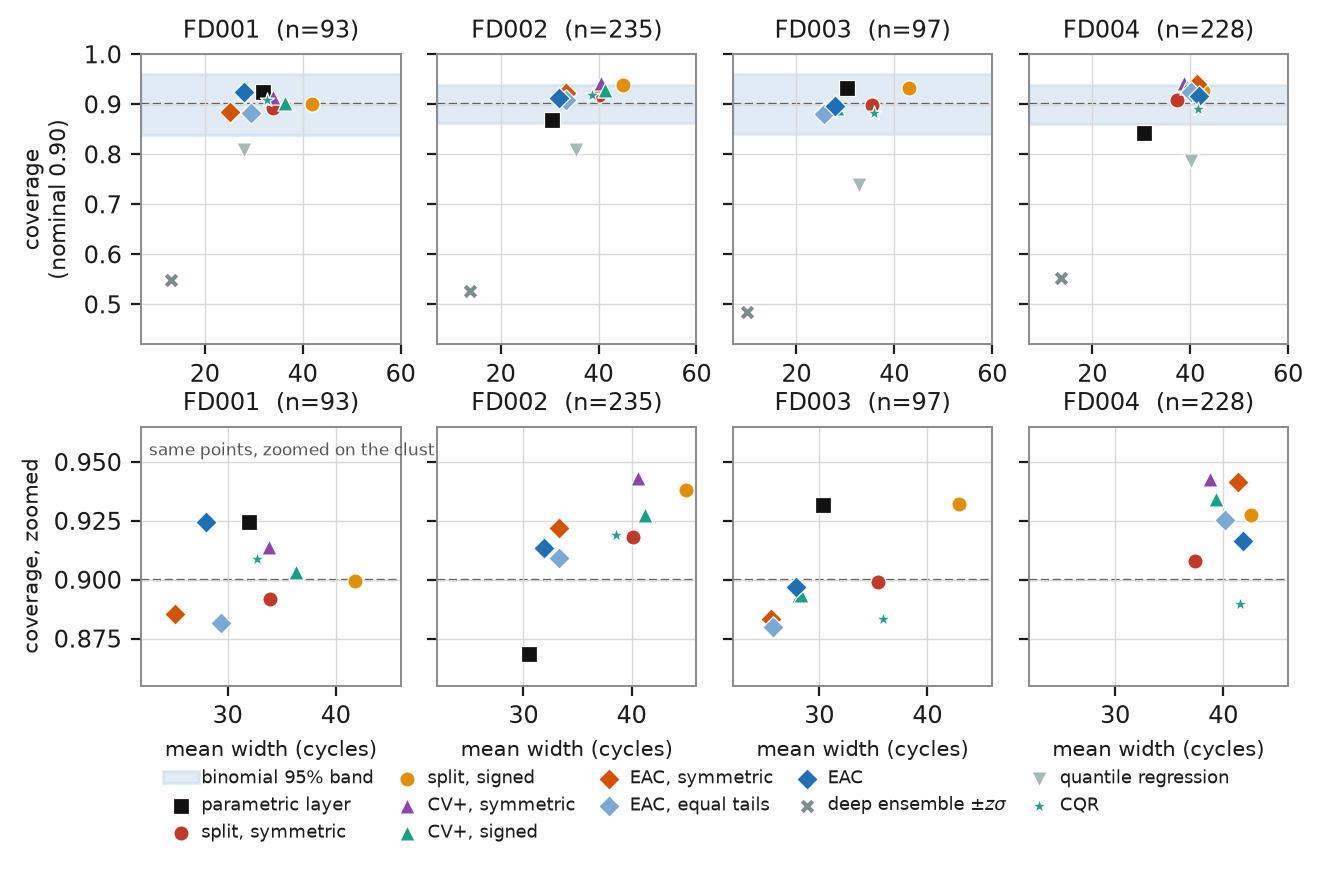
\includegraphics[width=\textwidth]{fig1_coverage_width.png}
\caption{Coverage against width at nominal 0.90, one panel per fleet. Top row: the full range,
including the two constructions that need no calibration (grey); the shaded band is the
binomial 95\,\% interval for a true coverage of 0.90 at that $n$. Bottom row: the same points
with the axes narrowed to the conformal cluster. Uncalibrated ensemble spread sits half a fleet
below nominal at a third of the width, and the calibrated constructions sit inside the band:
coverage cannot separate them at this scale, while width separates them by 30\,\%.}
\label{fig:plane}
\end{figure*}

\begin{figure}[t]
\centering
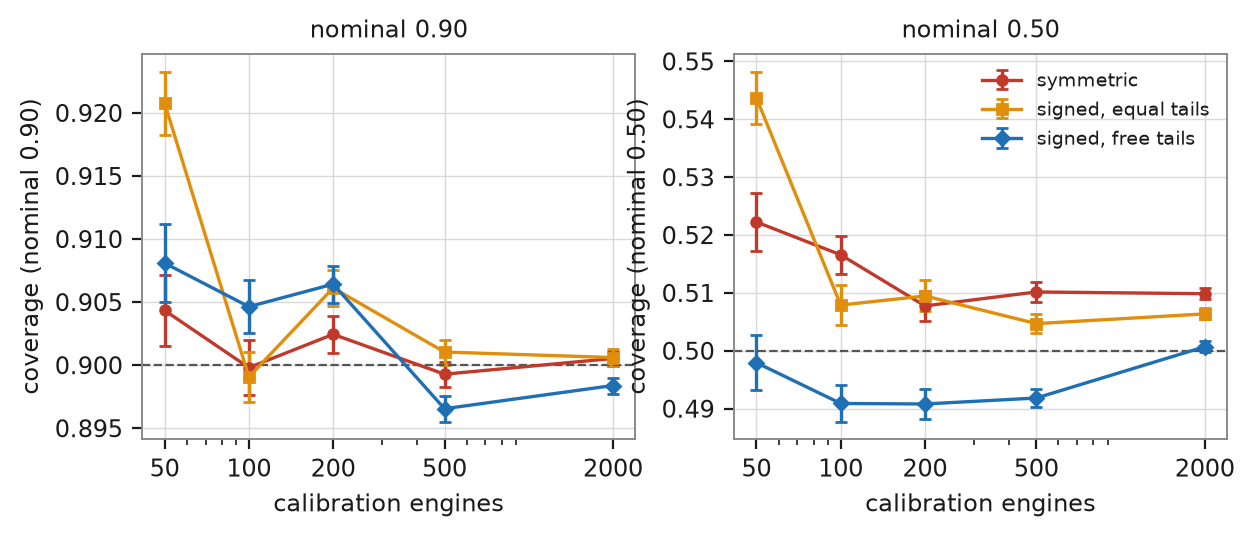
\includegraphics[width=\columnwidth]{fig2_simulation.png}
\caption{Simulation with known truth: coverage against the number of calibration engines, at
nominal 0.90 (left) and 0.50 (right). All three constructions are valid; they differ in width
by 16--21\,\% (not shown).}
\label{fig:sim}
\end{figure}

\section{Discussion}\label{sec:discussion}

\subsection{Why coverage tables cannot rank methods at this scale}

Fig.~\ref{fig:plane} makes the argument visually. At $n=93$ the 95\,\% band around a true 0.90
is $\pm 0.06$; at $n=235$ it is $\pm 0.04$. Every construction in Table~\ref{tab:main} except
the layer lies inside the band on at least three of four fleets, and two constructions that
differ by 30\,\% in width are indistinguishable on coverage. A table that reports
`PICP 0.912 versus 0.907' is therefore reporting sampling noise, not evidence, unless the
comparison is paired and the discordance is reported.

The detectability calculation in Table~\ref{tab:detect} makes the same point quantitatively and
in advance of any experiment: with 11--82 engines per bin, the smallest detectable deviation is
0.14--0.44. The five-bin comparison that a conditional-coverage table implies requires 149
engines per bin for a 10-point effect, and 516 for a 5-point effect. Pooling all four fleets
gives 84--212 per bin, which is enough for a 0.08--0.14 effect on the most populated bin and
nothing on the least.

\subsection{What to report}

We suggest four rules, each of which is a measurement fix rather than a modelling choice.
(i) Report coverage with its interval, and report the number of engines, not only the rate.
(ii) Use randomised PIT for distributions; the integer rule is biased upward by 0.01--0.04 at
0.90 and 0.07--0.12 at 0.50.
(iii) Report width, which is measurable to $\pm 1$ cycle and separates methods that coverage
cannot, and report it per fleet, because the fleet is a larger source of variation than the
method ($|\Delta|$ 0.09 across fleets for the layer versus 0.02 between constructions).
(iv) State which object was calibrated. If the deployed predictor is an ensemble, a
single-model conformal score is not the same object, and the difference is 11\,\% of the width.

\subsection{Limitations}

The study covers two simulated turbofan benchmarks and one backbone per benchmark. Both are
run-to-failure simulations, so the residual laws may be gentler than those of instrumented
machinery; the N-CMAPSS contrast suggests the direction of the difference (diffuse residuals,
where free tails win by 19\,\%) but does not establish it for real sensor data. The 50\,\%
level is not resolved on C-MAPSS by any construction, and we have not found a construction that
resolves it; we report the failure rather than selecting the seed that hides it. Finally, the
guarantees are marginal, and the paper's own detectability analysis is the reason we do not
claim conditional ones.

\section{Conclusion}\label{sec:concl}

RUL intervals are reported as a coverage and a width, and this paper has separated the part of
each that is information from the part that is convention. On 653 C-MAPSS engines and 2\,587
N-CMAPSS queries: the integer-endpoint convention inflates coverage by 0.011--0.044 at 0.90;
the central-interval convention costs 10.4\,\% of width; calibrating a fold model instead of
the deployed ensemble costs 11\,\%; and the benchmarks can detect only 0.14--0.44 deviations per
bin, which is larger than the differences that published tables rank. A matched-object
construction recovers the layer's sharpness (32.4 versus 30.9 cycles) with three times its
fleet stability ($|\Delta|$ 0.014 versus 0.037) and without its distributional assumptions,
and reaches nominal coverage on the independent benchmark where the parametric layer does not.
The broader conclusion is that the field's uncertainty numbers are now limited by measurement
practice more than by modelling: the same 653 engines that cannot resolve a 3-point coverage
difference can resolve a 10\,\% width difference, so width and its conventions are where the
next improvements will be visible.

\begin{table}[t]
\centering
\caption{Coverage bias of the integer-endpoint rule on the frozen layer, and the smallest
coverage deviation a bin can detect. Left: same predictive distribution, two conventions.
Right: $\dx$ at family-wise $\alpha=0.05$ over five bins and 80\,\% power.}
\label{tab:convention}
\begin{tabular}{lcccc}
\toprule
 & \multicolumn{2}{c}{bias at 0.90} & \multicolumn{2}{c}{bias at 0.50}\\
\cmidrule(lr){2-3}\cmidrule(lr){4-5}
Fleet & PIT & integer & PIT & integer\\
\midrule
FD001 & 0.924 & 0.935 & 0.517 & 0.591\\
FD002 & 0.869 & 0.902 & 0.523 & 0.643\\
FD003 & 0.931 & 0.948 & 0.524 & 0.608\\
FD004 & 0.842 & 0.886 & 0.420 & 0.535\\
\midrule
bias & \multicolumn{2}{c}{$+0.011$ to $+0.044$} & \multicolumn{2}{c}{$+0.074$ to $+0.120$}\\
\bottomrule
\end{tabular}
\end{table}

\begin{table}[t]
\centering
\caption{What a bin can prove. Bin sizes are the five RUL strata of the test sets; $\dx$ is
computed at family-wise $\alpha=0.05$ over five bins with 80\,\% power.}
\label{tab:detect}
\begin{tabular}{lccccc}
\toprule
 & \multicolumn{5}{c}{engines per bin}\\
\cmidrule(lr){2-6}
Fleet & $[0,25)$ & $[25,50)$ & $[50,75)$ & $[75,100)$ & $[100,125]$\\
\midrule
FD001 & 19 & 11 & 13 & 22 & 28\\
FD002 & 58 & 29 & 31 & 45 & 72\\
FD003 & 15 & 14 & 20 & 18 & 30\\
FD004 & 49 & 30 & 26 & 41 & 82\\
pooled & 141 & 84 & 90 & 126 & 212\\
\midrule
\multicolumn{6}{l}{$\dx$ at $n=11$: 0.44 \quad $n=82$: 0.14 \quad $n=141$: 0.10 \quad $n=212$: 0.08}\\
\multicolumn{6}{l}{engines needed: 149 for $\dx=0.10$, 243 for 0.075, 516 for 0.05}\\
\bottomrule
\end{tabular}
\end{table}

\begin{thebibliography}{99}

\bibitem{crulp}
S.~Piao, R.~Huang, and F.~Tsung, ``CRULP: Reliable RUL estimation inspired by conformal
prediction,'' \emph{IEEE Trans. Instrum. Meas.}, vol.~74, Art.~3505411, 2025,
doi: 10.1109/TIM.2024.3522678.

\bibitem{piao2025}
S.~Piao, Y.~Wang, R.~Huang, D.~Wang, and F.~Tsung, ``Quantify uncertainty beyond covariate
shift in RUL estimation by conformal prediction,'' in \emph{Proc. IEEE 21st Int. Conf. Autom.
Sci. Eng. (CASE)}, 2025, doi: 10.1109/CASE58245.2025.11163867.

\bibitem{wang2025}
W.~Wang, Z.~Wang, Z.~Cai, C.~Hu, and S.~Si, ``Robust uncertainty quantification for online
remaining useful life prediction with randomly missing and partially faulty sensor data,''
\emph{Rel. Eng. Syst. Saf.}, vol.~262, 2025.

\bibitem{moccardi2025}
A.~Moccardi, C.~Conte, R.~C. Ghosh, and F.~Moscato, ``A robust conformal framework for
IoT-based predictive maintenance,'' \emph{Future Internet}, vol.~17, no.~6, Art.~244, 2025.

\bibitem{hou2025}
Y.~Hou, M.~Ragab, Y.~Wang, M.~Wu, A.~Alseiari, C.-K.~Kwoh, X.~Li, and Z.~Chen, ``Evidential
domain adaptation for remaining useful life prediction with incomplete degradation,''
\emph{IEEE Trans. Instrum. Meas.}, 2025, doi: 10.1109/TIM.2025.3551977.

\bibitem{yang2025}
N.~Yang, W.~Zhang, J.~Zhang, K.~Wang, Y.~Su, and Y.~Liu, ``A method for remaining useful life
prediction and uncertainty quantification of rolling bearings based on fault feature gain,''
\emph{IEEE Trans. Instrum. Meas.}, 2025, doi: 10.1109/TIM.2025.3534227.

\bibitem{wang2025svsdm}
X.~Wang, X.~Si, X.~Xi, and D.~Zhou, ``Adaptive remaining useful life prediction based on a
system-level variable structure degradation model,'' \emph{IEEE Trans. Instrum. Meas.},
vol.~74, Art.~no.~1011213, 2025, doi: 10.1109/TIM.2025.3573776.

\bibitem{kim2025}
E.~Kim, S.~Park, H.~Lee, S.~Ko, and E.~Hwang, ``Enhanced remaining useful life prediction for
turbofan engines using spatiotemporal Koopman dual-branch transformer,'' \emph{IEEE Trans.
Instrum. Meas.}, vol.~74, pp.~1--16, 2025, doi: 10.1109/TIM.2025.3625335.

\bibitem{zhou2025}
J.~Zhou, J.~Yang, S.~Xiang, and Y.~Qin, ``Remaining useful life prediction methodologies with
health indicator dependence for rotating machinery: A comprehensive review,'' \emph{IEEE
Trans. Instrum. Meas.}, vol.~74, pp.~1--19, 2025.

\bibitem{wu2025}
H.~Wu, Y.~Wang, Z.~Tian, and M.~J. Zuo, ``Query based learning via conformal uncertainty for
RUL prediction,'' in \emph{Proc. IEEE Int. Conf. Prognostics Health Manage. (ICPHM)}, 2025,
pp.~1--8.

\bibitem{noot2025}
J.-P. Noot, M.~Martin, and E.~Birmel\'e, ``LSTM and transformers based methods for remaining
useful life prediction considering censored data,'' \emph{Int. J. Prognostics Health Manage.},
vol.~16, no.~2, 2025, doi: 10.36001/ijphm.2025.v16i2.4260.

\bibitem{vovk2005}
V.~Vovk, A.~Gammerman, and G.~Shafer, \emph{Algorithmic Learning in a Random World}.
New York, NY, USA: Springer, 2005.

\bibitem{barber2021}
R.~F. Barber, E.~J. Cand\`es, A.~Ramdas, and R.~J. Tibshirani, ``Predictive inference with the
jackknife+,'' \emph{Ann. Statist.}, vol.~49, no.~1, pp.~486--507, 2021.

\bibitem{barber2023}
R.~F. Barber, E.~J. Cand\`es, A.~Ramdas, and R.~J. Tibshirani, ``Conformal prediction beyond
exchangeability,'' \emph{Ann. Statist.}, vol.~51, no.~2, pp.~816--845, 2023.

\bibitem{romano2019}
Y.~Romano, E.~Patterson, and E.~J. Cand\`es, ``Conformalized quantile regression,'' in
\emph{Adv. Neural Inf. Process. Syst.}, vol.~32, 2019.

\bibitem{tibshirani2019}
R.~J. Tibshirani, R.~F. Barber, E.~J. Cand\`es, and A.~Ramdas, ``Conformal prediction under
covariate shift,'' in \emph{Adv. Neural Inf. Process. Syst.}, vol.~32, 2019.

\bibitem{angelopoulos2023}
A.~N. Angelopoulos and S.~Bates, ``Conformal prediction: A gentle introduction,''
\emph{Found. Trends Mach. Learn.}, vol.~16, no.~4, pp.~494--591, 2023.

\bibitem{kuleshov2018}
V.~Kuleshov, N.~Fenner, and S.~Ermon, ``Accurate uncertainties for deep learning using
calibrated regression,'' in \emph{Proc. Int. Conf. Mach. Learn. (ICML)}, 2018, pp.~2796--2804.

\bibitem{saxena2008}
A.~Saxena, K.~Goebel, D.~Simon, and N.~Eklund, ``Damage propagation modeling for aircraft
engine run-to-failure simulation,'' in \emph{Proc. Int. Conf. Prognostics Health Manage.}, 2008.

\bibitem{saxena2010}
A.~Saxena \emph{et al.}, ``Metrics for offline evaluation of prognostic performance,''
\emph{Int. J. Prognostics Health Manage.}, vol.~1, no.~1, 2010.

\bibitem{arias2021}
M.~Arias Chao, C.~Kulkarni, K.~Goebel, and O.~Fink, ``Aircraft engine run-to-failure dataset
under real flight conditions for prognostics and diagnostics,'' \emph{Data}, vol.~6, no.~1,
Art.~5, 2021.

\bibitem{ginting2007}
T.~Gneiting and A.~E. Raftery, ``Strictly proper scoring rules, prediction, and estimation,''
\emph{J. Amer. Statist. Assoc.}, vol.~102, no.~477, pp.~359--378, 2007.

\bibitem{wilson1927}
E.~B. Wilson, ``Probable inference, the law of succession, and statistical inference,''
\emph{J. Amer. Statist. Assoc.}, vol.~22, no.~158, pp.~209--212, 1927.

\end{thebibliography}

\end{document}
